\index{examples|see{datasets}}
\index{graphs|see{plots}}\index{multicollinearity|see{collinearity}}

\setcounter{chapter}{0}
\chapter{Regression and the Normal Distribution}

{\small \textit{Chapter Preview}. Regression analysis is a
statistical method that is widely used in many fields of study, with
actuarial science being no exception. This chapter provides an
introduction to the role of the normal distribution in regression,
the use of logarithmic transformations in specifying regression
relationships and the sampling basis that is critical for inferring
regression results to broad populations of interest.}

\section{What is Regression Analysis?}\label{S1:Intro}

Statistics is about data. As a discipline, it is about the
collection, summarization and analysis of data to make statements
about the real world. When analysts collect data, they are really
collecting information that is quantified, that is, transformed to a
numerical scale. There are easy, well-understood rules for reducing
the data, using either numerical or graphical summary measures.
These summary measures can then be linked to a theoretical
representation, or model, of the data. With a model that is
calibrated by data, statements about the world can be made.

\marginparjed{Statistics is about the collection, summarization and
analysis of data to make statements about the real world.}

Statistical methods have had a major impact on several fields of study.

\begin{itemize}
\item In the area of data collection, the careful design of \emph{sample
surveys} is crucial to market research groups and to the auditing procedures
of accounting firms.

\item \emph{Experimental design} is a second subdiscipline devoted to data
collection. The focus of experimental design is on constructing methods of
data collection that will extract information in the most efficient way
possible. This is especially important in fields such as agriculture and
engineering where each observation is expensive, possibly costing millions
of dollars.

\item Other applied statistical methods focus on managing and predicting
data. \emph{Process control} deals with monitoring a process over time and
deciding when intervention is most fruitful. Process control helps manage
the quality of goods produced by manufacturers.

\item \emph{Forecasting} is about extrapolating a process into the future,
whether it be sales of a product or movements of an interest rate.
\end{itemize}

Regression analysis is a statistical method used to analyze data. As
we will see, the distinguishing feature of this method is the
ability to make statements about variables after having controlled
for values of known explanatory variables. Important as other
methods are, it is regression analysis that has been most
influential. To illustrate, an index of business journals,
ABI/INFORM, lists over \emph{twenty-four thousand} articles using
regression techniques over the thirty-year period 1978-2007. And
these are only the applications that were considered innovative
enough to be published in scholarly reviews!

Regression analysis of data is so pervasive in modern business that
it is easy to overlook the fact that the methodology is barely over
120 years old. Scholars attribute the birth of regression to the
1885 presidential address of Sir Francis Galton to the
anthropological section of the British Association of the
Advancement of Sciences. In that address, described in Stigler
(1986), Galton provided a description of regression and linked it to
\emph{normal curve} theory. His discovery arose from his studies of
properties of natural selection and inheritance.

\empexjed{Galton}\index{datasets!Galton heights}

To illustrate a data set that can be analyzed using regression
methods, Table \ref{T1:Galton} displays some data included in
Galton's 1885 paper.\ecaptionjed{Galton's 1885 Regression Data} This
table displays the heights of 928 adult children, classified by an
index of their parents' height. Here, all female heights were
multiplied by 1.08, and the index was created by taking the average
of the father's height and rescaled mother's height. Galton was
aware that the parents' and the adult child's height could each be
adequately approximated by a normal curve. In developing regression
analysis, he provided a single model for the joint distribution of
heights.

\begin{table}[h] \scalefont{0.9}
\caption{\label{T1:Galton} Galton's 1885 Regression Data}
\begin{tabular}{l|ccccccccccc|r}
\hline
Height of &  \multicolumn{12}{c}{Parents' Height} \\
\multicolumn{2}{l}{adult child} \\
in inches & $<$64.0 & 64.5 & 65.5 & 66.5 & 67.5 & 68.5 &
69.5 & 70.5 & 71.5 & 72.5 & $>$73.0 & Total \\
\hline
$>$73.7 & - & - & - & - & - & - & 5 & 3 & 2 & 4 & - & 14 \\
73.2 & - & - & - & - & - & 3 & 4 & 3 & 2 & 2 & 3 & 17 \\
72.2 & - & - & 1 & - & 4 & 4 & 11 & 4 & 9 & 7 & 1 & 41 \\
71.2 & - & - & 2 & - & 11 & 18 & 20 & 7 & 4 & 2 & - & 64 \\
70.2 & - & - & 5 & 4 & 19 & 21 & 25 & 14 & 10 & 1 & - & 99 \\
69.2 & 1 & 2 & 7 & 13 & 38 & 48 & 33 & 18 & 5 & 2 & - & 167 \\
68.2 & 1 & - & 7 & 14 & 28 & 34 & 20 & 12 & 3 & 1 & - & 120 \\
67.2 & 2 & 5 & 11 & 17 & 38 & 31 & 27 & 3 & 4 & - & - & 138 \\
66.2 & 2 & 5 & 11 & 17 & 36 & 25 & 17 & 1 & 3 & - & - & 117 \\
65.2 & 1 & 1 & 7 & 2 & 15 & 16 & 4 & 1 & 1 & - & - & 48 \\
64.2 & 4 & 4 & 5 & 5 & 14 & 11 & 16 & - & - & - & - & 59 \\
63.2 & 2 & 4 & 9 & 3 & 5 & 7 & 1 & 1 & - & - & - & 32 \\
62.2 & - & 1 & - & 3 & 3 & - & - & - & - & - & - & 7 \\
$<$61.2 & 1 & 1 & 1 & - & - & 1 & - & 1 & - & - & - & 5 \\ \hline
Total & 14 & 23 & 66 & 78 & 211 & 219 & 183 & 68 & 43 & 19 & 4 & 928 \\
\hline
\end{tabular}
\textit{Source: }Stigler (1986).
 \scalefont{1.1111}
\end{table}

\marginparjed{Regression analysis is a method to quantify the
relationship between a variable of interest and explanatory
variables.}

\index{explanatory variable}

Table \ref{T1:Galton} shows that much of the information concerning
the height of an adult child can be attributed to, or ``explained,''
in terms of the parents' height. Thus, we use the term
\emph{explanatory variable} for measurements that provide
information about a variable of interest. Regression analysis is a
method to quantify the relationship between a variable of interest
and explanatory variables. The methodology used to study the data in
Table \ref{T1:Galton} can also be used to study actuarial and other
risk management problems, the thesis of this book.

\section{Fitting Data to a Normal
Distribution}\index{distributions!normal}

Historically, the normal distribution had a pivotal role in the
development of regression analysis. It continues to play an
important role, although we will be interested in extending
regression ideas to highly ``non-normal'' data.

Formally, the normal curve is defined by the function
\begin{equation}\label{E1:Normalpdf}
\mathrm{f}(y)=\frac{1}{\sigma \sqrt{2\pi }}\exp \left( -\frac{1}{2\sigma ^{2}%
}\left( y-\mu \right) ^{2}\right) .
\end{equation}
\marginparjed{Appendix A3.1 provides additional details about the
normal curve, including a graph and distribution table.}

\noindent This curve is a probability density function with the
whole real line as its domain. From equation (\ref{E1:Normalpdf}),
we see that the curve is symmetric about $\mu $\ (the mean and
median). The degree of peakedness is controlled by the parameter
$\sigma ^{2}$. These two parameters, $\mu $\ and $\sigma ^{2}$, are
known as the \emph{location} and \emph{scale parameters},
respectively. Appendix A3.1 provides additional details about this
curve, including a graph and tables of its cumulative distribution
that we will use throughout the text.

The normal curve is also depicted in Figure \ref{F1:TenMarks}, a
display of a now out-of-date German currency note, the ten Deutsche
Mark. This note contains the image of German Carl Gauss, an eminent
mathematician whose name is often linked with the normal curve (it
is sometimes referred to as the \emph{Gaussian curve}). Gauss
developed the normal curve in connection with the theory of least
squares for fitting curves to data in 1809, about the same time as
related work by the French scientist Pierre LaPlace. According to
Stigler (1986), there was quite a bit of acrimony between these two
scientists about the priority of discovery! The normal curve was
first used as an approximation to histograms of data around 1835 by
Adolph Quetelet, a Belgian mathematician and social scientist. Like
many good things, the normal curve had been around for some time,
since about 1720 when Abraham de Moivre derived it for his work on
modeling games of chance. The normal curve is popular because it is
easy to use and has proved to be successful in many applications.

\begin{figure}[htp]
  \begin{center}
    \includegraphics[natheight=5in, natwidth=8in, height=2in, width=4in]
    {Chapter1/GreyScale256TenDM.jpg}
    \caption{\label{F1:TenMarks} \small Ten Deutsche Mark - German currency featuring scientist Gauss and the normal curve .}
  \end{center}
\end{figure}

\bigskip

\linejed

\empexjed{MassBodilyInjury}\index{datasets!Massachusetts bodily
injury claims}

\textbf{Example: Massachusetts Bodily Injury Claims.}
\ecaptionjed{Massachusetts Bodily Injury Claims} For our first look
at fitting the normal curve to a set of data, we consider data from
Rempala and Derrig (2005). They considered claims arising from
automobile bodily injury insurance coverages. These are amounts
incurred for outpatient medical treatments that arise from
automobile accidents, typically sprains, broken collarbones and the
like. The data consists of a sample of 272 claims from Massachusetts
that were closed in 2001 (by ``closed,'' we mean that the claim is
settled and no additional liabilities can arise from the same
accident). Rempala and Derrig were interested in developing
procedures for handling mixtures of ``typical'' claims and others
from providers who reported claims fraudulently. For this sample, we
consider only those typical claims, ignoring the potentially
fraudulent ones.\index{actuarial \& financial terms and
concepts!closed claim}

Table \ref{T1:BISummaryStats} provides several statistics that
summarize different aspects of the distribution. Claim amounts are
in units of logarithms of thousands of dollars. The average
logarithmic claim is 0.481, corresponding to \$1,617.77 (=1000 $\exp
(0.481)$). The smallest and largest claims are -3.101 (\$45) and
3.912 (\$50,000), respectively.

\bigskip

\begin{table}[h]
\scalefont{0.9} \caption{\label{T1:BISummaryStats} Summary
Statistics of Massachusetts Automobile Bodily Injury Claims}
\begin{tabular}{l|cccccccc}
\hline
Variable &  &  &  & Standard &  &  & 25th & 75th \\
& Number & Mean & Median & Deviation & Minimum & Maximum &
Percentile & Percentile  \\ \cline{2-9} \vspace{-.05in} \\
Claims & 272 & 0.481 & 0.793 & 1.101 & -3.101 & 3.912 & -0.114 & 1.168 \\
\hline
\multicolumn{9}{l}{\textit{Note: }Data are in logs of thousands of dollars}%
\end{tabular}
 \scalefont{1.1111}

\linetjed
\end{table}

For completeness, here are a few definitions. The \emph{sample} is
the set of data available for analysis, denoted by $y_1,...,y_n$.
Here, $n$ is the number of observations, $y_1$ represents the first
observation, $y_2$ the second, and so on up to $y_n$ for the $nth$
observation. Here are a few important summary statistics.

\bigskip\index{symbols!$\bar{y}$, sample mean}
\index{symbols!$s_y$, sample standard deviation} \index{symbols!$n$,
sample size}\index{symbols!$y$, observed variable, typically the
outcome of interest}


\boxedjed

\textit{Basic Summary Statistics} \enumerate
\item The
\emph{mean} is the average of observations, that is, the sum of the
observations divided by the number of units. Using algebraic
notation, the mean is\
\begin{equation*}
\overline{y}=\frac{1}{n}\left( y_1 + \cdots + y_n \right) =
\frac{1}{n} \sum_{i=1}^{n} y_i.
\end{equation*}

\item The \emph{median} is the middle observation when the observations are ordered by
size. That is, it is the observation at which 50\% are below it (and
50\% are above it).

\item The \emph{standard deviation} is a measure of the spread, or scale, of
the distribution. It is computed as
\begin{equation*}
s_y = \sqrt{\frac{1}{n-1}\sum_{i=1}^{n}\left(
y_i-\overline{y}\right) ^{2}} .
\end{equation*}

\item A \emph{percentile} is a number at which a specified fraction of the
observations is below it, when the observations are ordered by size.
For example, the 25th percentile is that number so that 25\% of
observations are below it.
\end{boxedminipage}

\bigskip\index{plots!histogram}

To help visualize the distribution, Figure \ref{F1:BIHist} displays
a \emph{histogram} of the data. Here, the height of the each
rectangle shows the relative frequency of observations that fall
within the range given by its base. The histogram provides a quick
visual impression of the distribution; it shows that the range of
the data is approximately (-4,4), the central tendency is slightly
greater than zero and that the distribution is roughly symmetric.

\bigskip

\textbf{Normal Curve Approximation.} Figure \ref{F1:BIHist} also
shows a normal curve superimposed, using $\overline{y}$ for $\mu $
and $s_y^{2}$ for $\sigma ^{2}$. With the normal curve, only two
quantities ($\mu $ and $\sigma ^{2}$) are required to summarize the
entire distribution. For example, Table \ref{T1:BISummaryStats}
shows that 1.168 is the 75th percentile, which is approximately the
204th (= .$75\times 272$) largest observation from the entire
sample. From the equation (\ref{E1:Normalpdf}) normal distribution,
we have that $z=(y-\mu )/\sigma $ is a standard normal, of which
0.675\ is the 75th percentile. Thus, $\overline{%
y}+0.675s_y=0.481+0.675\times 1.101=1.224$ is the 75th percentile
using the normal curve approximation.


\begin{figure}[htp]
    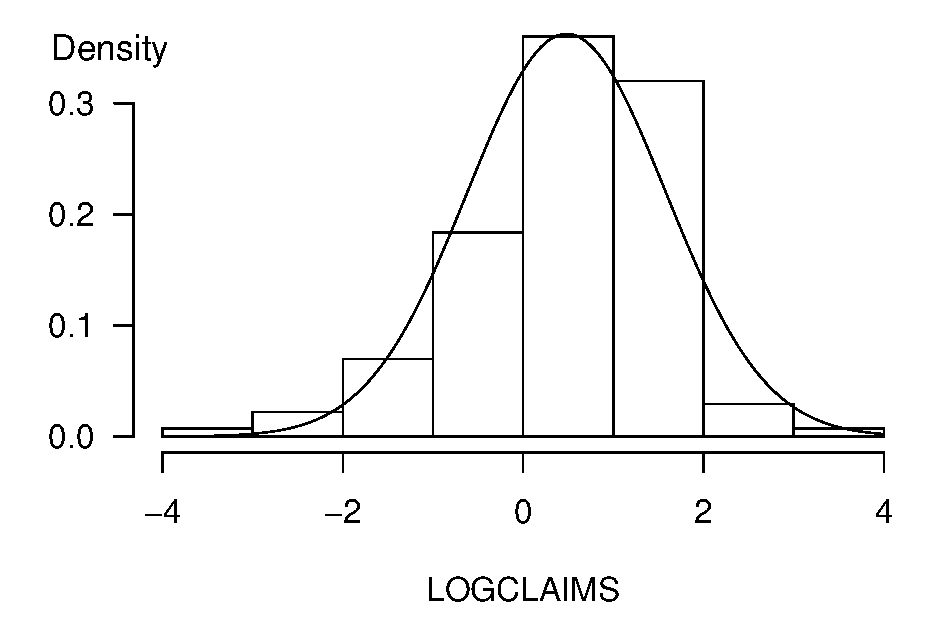
\includegraphics[width=0.45\textwidth]
        {Chapter1/F1BIHist.eps} \hfill  $~~~$
               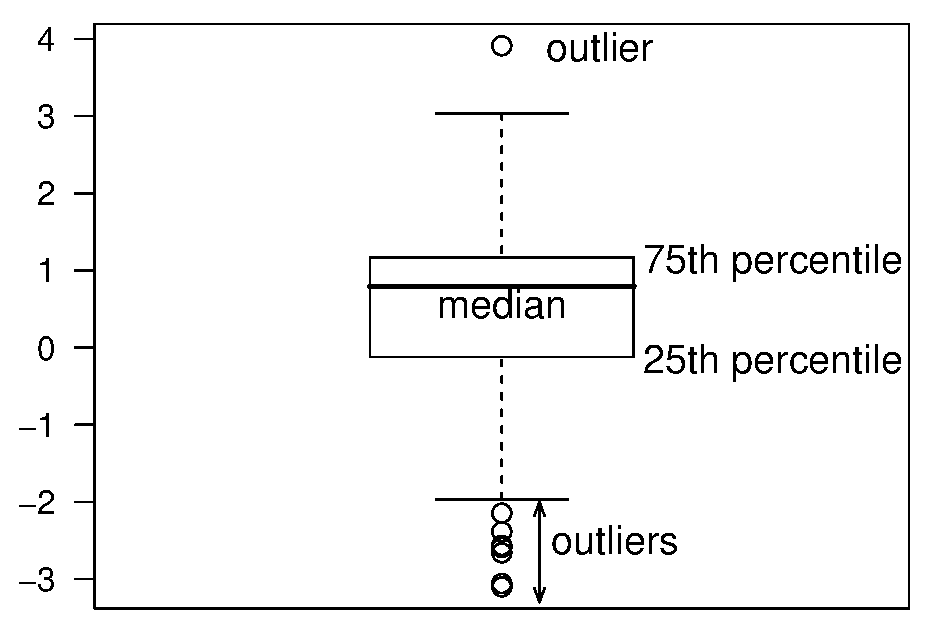
\includegraphics[width=0.45\textwidth]
        {Chapter1/F1BoxPlot.eps}

      \parbox[t]{2.5in}{\caption{\label{F1:BIHist} \small Bodily Injury Relative Frequency with Normal Curve
                Superimposed.}} \hfill
        \parbox[t]{2.5in}{\caption{\label{F1:BoxPlot} \small Box Plot of Bodily Injury
        Claims.}}
\end{figure}


\bigskip\index{plots!box and whiskers}

\textbf{Box Plot. \ }A quick visual inspection of a variable's
distribution can reveal some surprising features that are hidden by
statistics, numerical summary measures. The \emph{box plot}
\index{plots!box}, also known as a ``box and whiskers'' plot, is one
such graphical device. Figure \ref{F1:BoxPlot} illustrates a box
plot for the bodily injury claims. Here, the box captures the middle
50\% of the data, with the three horizontal lines corresponding to
the 75th, 50th and 25th percentiles, reading from top to bottom. \
The horizontal lines above and below the box are the ``whiskers.''
The upper whisker is 1.5 times the \emph{interquartile range} (the
difference between the 75th and 25th percentiles) above the 75th
percentile. Similarly, the lower whisker is 1.5 times the
interquartile range below the 25th percentile. Individual
observations outside the whiskers are denoted by small circular
plotting symbols, and are referred to as ``outliers.''

\bigskip

Graphs are powerful tools; they allow analysts to readily visualize
nonlinear relationships that are hard to comprehend when expressed
verbally or by mathematical formula. However, by their very
flexibility, graphs can also readily deceive the analyst. Chapter 21
will underscore this point. For example, Figure
\ref{F1:BIHistRedraw} is a re-drawing of Figure \ref{F1:BIHist}; the
difference is that Figure \ref{F1:BIHistRedraw} uses more, and
finer, rectangles. This finer analysis reveals the asymmetric nature
of the sample distribution that was not evident in Figure
\ref{F1:BIHist}.


\bigskip

\textbf{Quantile-Quantile Plots.} Increasing the number of
rectangles can unmask features that were not previously apparent;
however, there are in general fewer observations per rectangle
meaning that the uncertainty of the relative frequency estimate
increases. This represents a trade-off. Instead of forcing the
analyst to make an arbitrary decision about the number of
rectangles, an alternative is to use a graphical device for
comparing a distribution to another known as a
\emph{quantile-quantile}, or \emph{qq},
plot.\index{plots!quantile-quantile, $qq$}

Figure \ref{F1:BIQQPlot} illustrates a $qq$ plot for the bodily
injury data using the normal curve as a reference distribution. For
each point, the vertical axis gives the quantile using the sample
distribution. The horizontal axis gives the corresponding quantity
using the normal curve. For example, earlier we considered the 75th
percentile point. This point appears as (1.168, 0.675) on the graph.
To interpret a $qq$ plot, if the quantile points lie along the
superimposed line, then the sample and the normal reference
distribution have the same shape. (This line is defined by
connecting the 75th and 25th percentiles.)

\marginparjed{Points in a $qq$ plot close to a straight line
suggests agreement between the sample and reference distributions.}

In Figure \ref{F1:BIQQPlot}, the small sample percentiles are
consistently smaller than the corresponding values from the standard
normal, indicating that the distribution is skewed to the left. The
difference in values at the ends of the distribution are due to the
outliers noted earlier that could also be interpreted as the sample
distribution having larger tails than the normal reference
distribution.




\begin{figure}[htp]
  \begin{center}
    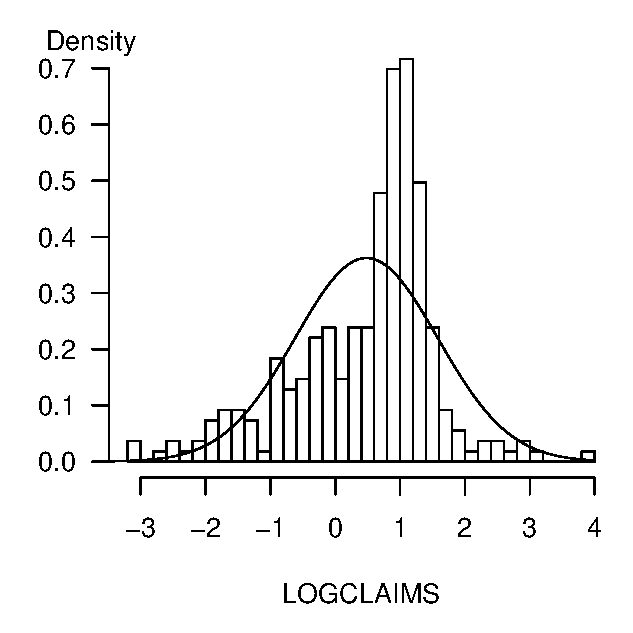
\includegraphics[width=0.45\textwidth]
        {Chapter1/F1BIHistRedraw.eps}
      \hfill
            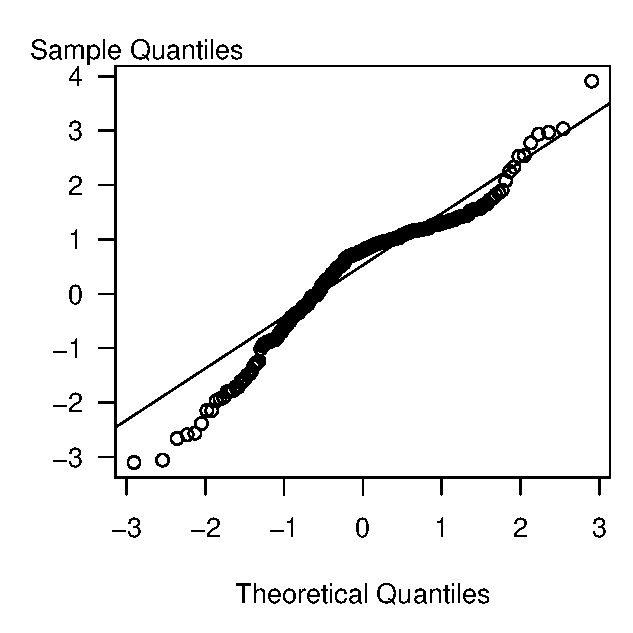
\includegraphics[width=0.45\textwidth]
        {Chapter1/F1BIQQPlot.eps}

      \end{center}
           \parbox[t]{2.5in}{\caption {\label{F1:BIHistRedraw}
           {\small Re-drawing of Figure \ref{F1:BIHist} with an increased number of rectangles.}}} \hfill
        \parbox[t]{2.5in}{\caption {\label{F1:BIQQPlot} {\small A $qq$ plot of
Bodily Injury Claims, using a normal reference distribution.}}}

\end{figure}


\section{Power Transforms}\label{S1:PowerTransforms}\index{transformations!power}

In the Section 1.2 example, we considered claims without justifying
the use of the logarithmic scaling. When analyzing variables such as
assets of firms, wages of individuals and housing prices of
households in business and economic applications, it is common to
consider logarithmic instead of the original units. A log transform
retains the original ordering (for example, large wages remain large
on the log wage scale) but serves to ``pull in'' extreme values of
the distribution.

To illustrate, Figure \ref{F1:BIOrig} shows the bodily injury claims
distribution in (thousands of) dollars. In order to graph the data
meaningfully, the largest observation (\$50,000) was removed prior
to making this plot. Even with this observation removed, Figure
\ref{F1:BIOrig} shows that the distribution is heavily lop-sided to
the right, with several large values of claims appearing.
\index{transformations!logarithmic}


\marginparjed{A right-skewed distribution is has long tails on the
right and a concentration of mass on the left. Many insurance claims
distributions are right-skewed.}

Distributions that are lopsided in one direction or the other are
known as \emph{skewed}. Figure \ref{F1:BIOrig} is an example of a
distribution skewed to the right, or positively skewed. Here, the
tail of the distribution on the right is longer and there is a
greater concentration of mass to the left. In contrast, a
left-skewed, or negatively skewed distribution, has a longer tail on
the left and a greater concentration of mass to the right. Many
insurance claims distributions are right-skewed (see the text by
Klugman, Panjer and Willmot, 2008, for extensive discussions). As we
saw in Figures \ref{F1:BIHistRedraw} and \ref{F1:BIQQPlot}, a
logarithmic transformation yields a distribution that is only mildly
skewed to the left.


\setcounter{figure}{5}

\begin{figure}[htp]
  \begin{center}
    
\includegraphics[width=.4\textwidth]
        {Chapter1/F1BIOrig.eps}
    \caption{\label{F1:BIOrig} \small Distribution of Bodily Injury Claims. Observations are in (thousands of)
dollars with the largest observation omitted.}
  \end{center}
\end{figure}

\index{transformations!Box-Cox family}

Logarithmic transformations are used extensively in applied
statistics work. One advantage is that they serve to symmetrize
distributions that are skewed. More generally, we consider
\emph{power transforms}, also known as the \emph{Box-Cox family of
transforms}. Within this family of transforms, in lieu of using the
response $y$, we use a transformed, or rescaled version, $y^{\lambda
}$. Here, the power $\lambda $ (lambda, a Greek ``el'') is a number
that may be user specified. Typical values of $\lambda $ that are
used in practice are $\lambda $=1, 1/2, 0 or -1. When we use
$\lambda =0$, we mean $\ln (y)$, that is, the natural logarithmic
transform. More formally, the Box-Cox family can be expressed as
\begin{equation*}
y^{(\lambda )}=\left\{
\begin{array}{ll}
\frac{y^{\lambda }-1}{\lambda } & \lambda \neq 0 \\
\ln (y) & \lambda =0
\end{array}
\right. .
\end{equation*}
As we will see, because regression estimates are not affected by
location and scale shifts, in practice we do not need to subtract
one nor divide by $\lambda $ when rescaling the response. The
advantage of the above expression is that, if we let $\lambda $
approach 0, then $y^{(\lambda )}$ approaches $\ln (y)$, from some
straightforward calculus arguments.

To illustrate the usefulness of transformations, we simulated 500
observations from a chi-square distribution with two degrees of
freedom. Appendix A3.2 introduces this distribution (that we will
encounter again later in studying the behavior of test statistics).
The upper left panel of Figure \ref{F1:ChiSquare} shows the original
distribution is heavily skewed to the right. The other panels in
Figure \ref{F1:ChiSquare} show the data rescaled using the square
root, logarithmic and negative reciprocal transformations. The
logarithmic transformation, in the lower left panel, provides the
best approximation to symmetry for this example. The negative
reciprocal transformation is based on $\lambda =-1$, and then
multiplying the rescaled observations by minus one, so that large
observations remain large.\index{distributions!chi-square}


\begin{figure}[htp]
  \begin{center}
    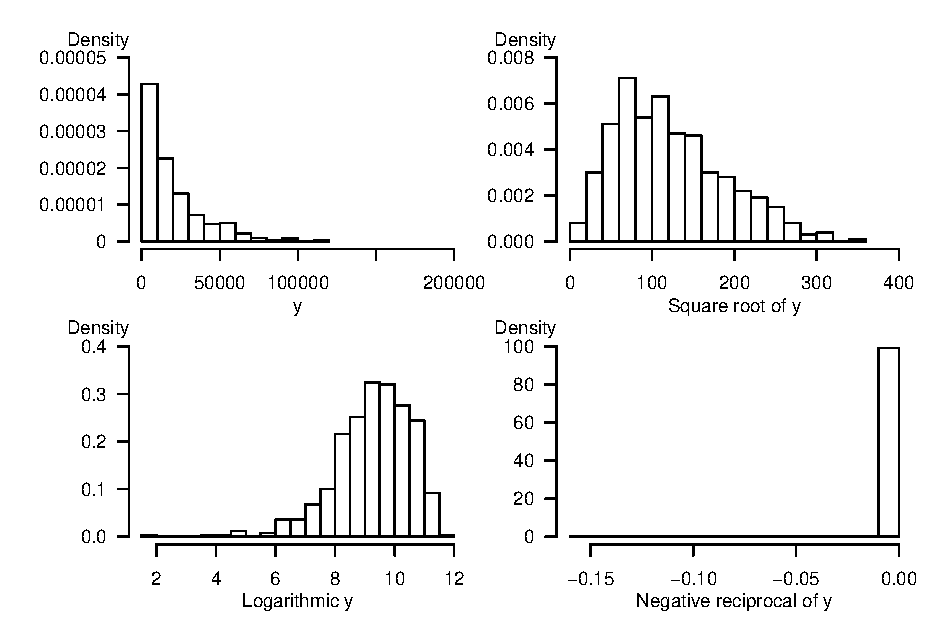
\includegraphics[width=1\textwidth]
        {Chapter1/F1Chisquare.eps}
    \caption{\label{F1:ChiSquare} \small 500
simulated observations from a chi-square distribution. The upper
left panel is based on the original distribution. The upper right
corresponds to the square root transform, the lower left to the log
transform and the lower right to the negative reciprocal transform.}
  \end{center}
\end{figure}


\section{Sampling and the Role of Normality}

\index{statistic}

A \emph{statistic} is a summary measure of data, such as a mean,
median or percentile. Collections of statistics are very useful for
analysts, decision-makers and everyday consumers for understanding
massive amounts of data that represent complex situations. To this
point, our focus has been on introducing sensible techniques to
summarize variables; techniques that will be used repeatedly thought
this text. However, the true usefulness of the \emph{discipline of
statistics} is its ability to say something about the unknown, not
merely to summarize information already available. To this end, we
need to make some fairly formal assumptions about the manner in
which the data are observed. As a science, a strong feature of
statistics (as a discipline) is the ability to critique these
assumptions and offer improved alternatives in specific situations.

\marginparjed{A statistic is a summary measure of a sample.
Statistics, as a discipline, can be used to infer behavior about a
larger population from a sample.}

\index{model assumptions}\index{symbols!$\mu$, population mean}
\index{symbols!$\sigma^2$, population
variance}\index{symbols!$\sigma$, population standard deviation}
\index{symbols!E , expectation operator}\index{symbols!Var ,
variance operator}

It is customary to assume that the data are drawn from a larger
population that we are interested in describing. The process of
drawing the data is known as the \emph{sampling}, or \emph{data
generating, process}. We denote this sample as $\{y_1,\ldots,y_n\}$.
So that we may critique, and modify, these sampling assumptions, we
list them below in detail:\smallskip

\begin{center}
\begin{tabular}{l}
\hline \textit{Basic Sampling Assumptions} \\ \hline
1. $\mathrm{E~}y_i=\mu $ \\
2. $\mathrm{Var~}y_i=\sigma ^{2}$ \\
3. $\{y_i\}$ are independent \\
4. $\{y_i\}$ are normally distributed. \\ \hline
\end{tabular}
\end{center}

\marginparjed{Assumption 4 is not required for many statistical
inference procedures because central limit theorems provide
approximate normality for many statistics of interest.}

In this basic set-up, $\mu $\ and $\sigma ^{2}$\ serve as
\emph{parameters} that describe the location and scale of the parent
population. The goal is to infer something sensible about them based
on statistics such as $\overline{y}$ and $s_y^{2}$. For the third
assumption, we assume independence among the draws. In a sampling
scheme, this may be guaranteed by taking a simple random sample from
a population. The fourth assumption is not required for many
statistical inference procedures because central limit theorems
provide approximate normality for many statistics of interest.
However, a formal justification of some statistics, such as
\textit{t}-statistics, requires this additional
assumption.\index{theorems!central limit}

Section \ref{S1:TechSupp} provides an explicit statement of one
version of the central limit theorem, giving conditions under which
$\overline{y}$ is approximately normally distributed. This section
also discusses a related result, known as an \emph{Edgeworth
approximation}, that shows that the quality of the normal
approximation is better for symmetric parent populations when
compared to skewed distributions.

\marginparjed{Linear regression is the study of weighted averages.}

How does this discussion apply to the study of regression analysis?
After all, so far we have focused only on the simple arithmetic
average, $\overline{y}$. In subsequent chapters, we will emphasize
that \emph{linear regression is the study of weighted averages};
specifically, many regression coefficients can be expressed as
weighted averages with appropriately chosen weights. Central limit
and Edgeworth approximation theorems are available for weighted
averages - these results will ensure approximate normality of
regression coefficients. To use normal curve approximations in a
regression context, we will often transform variables to achieve
approximate symmetry.

\marginparjed{We often transform variables to achieve approximate
symmetry to use normal curve approximations in a regression
context.}

\section{Regression and Sampling Designs}

Approximating normality will be an important issue in practical
applications of linear regression. Parts I and II of this book focus
on linear regression, where we will learn basic regression concepts
and sampling design. Part III will focus on \emph{nonlinear}
regression, involving binary, count and fat-tailed responses, where
the normal is not the most helpful reference distribution. Ideas
concerning basic concepts and design will also be used in the
nonlinear setting.

In regression analysis, we focus on one measurement of interest and
call this the \emph{dependent variable}. Other measurements are used
as \emph{explanatory variables}. A goal is to compare differences in
the dependent variable in terms of differences in the explanatory
variables. As noted in Section \ref{S1:Intro}, regression is used
extensively in many scientific fields. Table
\ref{T1:RegressionTerms} lists alternative terms that you may
encounter as you read regression applications.

\index{explanatory variable!independent variable}\index{explanatory
variable!regressor}\index{explanatory
variable!predictor}\index{explanatory variable!right-hand side}
\index{explanatory variable!exogenous}

\index{dependent variable}\index{dependent variable!outcome of
interest}\index{dependent variable!endogenous}\index{dependent
variable!response}\index{dependent
variable!regressand}\index{dependent variable!left-hand
side}\index{dependent variable!explained}

\begin{table}[h] \scalefont{0.9}
\caption{\label{T1:RegressionTerms} Terminology for Regression
Variables}
\begin{tabular}{ll}
\hline \multicolumn{1}{c}{$y$-variable} & \multicolumn{1}{c}{$x$-variable} \\
Outcome of interest & Explanatory variable \\
Dependent variable & Independent variable \\
Endogenous variable & Exogenous variable \\
Response & Treatment \\
Regressand & Regressor \\
Left-hand side variable & Right-hand side variable \\
Explained variable & Predictor variable \\
Output & Input \\
 \hline
\end{tabular}\scalefont{1.1111}\end{table}



In the latter part of the nineteenth century and early part of the
twentieth century, statistics was beginning to make an important
impact on the development of experimental science. Experimental
sciences often use \emph{designed studies}, where the data are under
the control of an analyst. Designed studies are performed in
laboratory settings, where there are tight physical restrictions on
every variable that a researcher thinks may be important. Designed
studies also occur in larger field experiments, where the mechanisms
for control are different than in laboratory settings. Agriculture
and medicine use designed studies. Data from a designed study are
said to be \emph{experimental data}.

\marginparjed{In designed studies, the data are under the control of
an analyst. Data from a designed study are said to be experimental
data.}

To illustrate, a classic example is to consider the yield of a crop
such as corn, where each of several parcels of land (the
observations) are assigned various levels of fertilizer. The goal is
ascertain the effect of fertilizer (the explanatory variable) on the
corn yield (the response variable). Although researchers attempt to
make parcels of land as much alike as possible, differences
inevitably arise. Agricultural researchers use \emph{randomization
techniques} to assign different levels of fertilizer to each parcel
of land. In this way, analysts can explain the variation in corn
yields in terms of the variation of fertilizer levels. Through the
use of randomization techniques, researchers using designed studies
can infer that the treatment has a \emph{causal effect} on the
response. Chapter 6 discusses causality further.

\linejed \index{examples!Rand health insurance
experiment}\index{actuarial \& financial terms and concepts!demand}

\textbf{Example: Rand Health Insurance Experiment}. How are medical
care expenditures related to the demand for insurance? Many studies
have established a positive relation between the amount spent on
medical care and the demand for health insurance. Those in poor
health anticipate using more medical services than similarly
positioned people in good or fair health and will seek higher levels
of health insurance to compensate for these anticipated
expenditures. They obtain this additional health insurance by (i)
selecting a more generous health insurance plan from an employer,
(ii) choosing an employer with a more generous health insurance plan
or (iii) paying more for individual health insurance. Thus, it is
difficult to disentangle the cause and effect relationship of
medical care expenditures and the availability of health insurance.

A study reported by Manning et al. (1987) sought to answer this
question using a carefully designed experiment. In this study,
enrolled households from six cities, between November 1974 and
February 1977, were \emph{randomly assigned} to one of 14 different
insurance plans. These plans varied by the cost-sharing elements,
the co-insurance rate (the percentage paid on out-of-pocket
expenditures which varied by 0, 25, 50 and 95\%) as well as the
deductible (5, 10 or 15 percent of family income, up to a maximum of
\$1,000). Thus, there was a \emph{random} assignment to levels of
the treatment, the amount of health insurance. The study found that
more favorable plans resulted in greater total expenditures, even
after controlling for participants' health status.

\linejed

\bigskip

For actuarial science and other social sciences, designed studies
are the exception rather than the rule. For example, if we want to
study the effects of smoking on mortality, it is highly unlikely
that we could get study participants to agree to be randomly
assigned to smoker/nonsmoker groups for several years just so that
we could observe their mortality patterns! As with the Section
\ref{S1:Intro} Galton study, social science researchers generally
work with \emph{observational data}. Observational data are not
under control of the analyst.

With observational data, we can not infer causal relationships but
we can readily introduce measures of \emph{association}. To
illustrate, in the Galton data, it is apparent that ``tall'' parents
are likely to have ``tall'' children and conversely ``short''
parents are likely to have ``short'' children. Chapter 2 will
introduce a correlation and other measures of association. However,
we can not infer causality from the data. For example, there may be
another variable, such as family diet, that is related to both
variables. Good diet in the family could be associated with tall
heights of parents and adult children, whereas poor diet stifles
growth. If this were the case, we would call family diet a
\emph{confounding variable}.

\marginparjed{With statistical control, we seek to compare a $y$ and
an $x$, ``controlling for'' the effects of other explanatory
variables.}

In designed experiments such as the Rand Health Insurance
Experiment, we can control for the effects of variables such as
health status through random assignment methods. In observational
studies, we use \emph{statistical control}, rather than experimental
control. To illustrate, for the Galton data, we might split our
observations into two groups, one for ``good family diet'' and one
for ``poor family diet,'' and examine the relationship between
parents' and children's height for each subgroup. This is the
essence of the regression method, to compare a $y$ and an $x$,
``controlling for'' the effects of other explanatory variables.

Of course, to use statistical control and regression methods, one
must record family diet, and any other measures of height that may
confound the effects of parents' height on the height of their adult
child. The difficulty in designing studies is trying to imagine all
of the variables that could possibly affect a response variable, an
impossible task in most social science problems of interest. To give
some guidance on when ``enough is enough,'' Chapter 6 will discuss
measures of an explanatory variable's importance and its impact on
model selection.

\section{Actuarial Applications of Regression}

This book introduces a statistical method, regression analysis. The
introduction is organized around the traditional triad of
statistical inference:
\begin{itemize}
\item hypothesis testing,
\item estimation and
\item prediction.
\end{itemize}
Further, this book shows how this methodology can be used in
applications that are likely to be of interest to actuaries and to
other risk analysts. As such, it is helpful to begin with the three
traditional areas of actuarial applications:
\begin{itemize}
\item pricing,
\item reserving and
\item solvency testing.
\end{itemize}

\index{actuarial \& financial terms and concepts!adverse selection}
\index{actuarial \& financial terms and concepts!pricing}

\textbf{Pricing and adverse selection.} Regression analysis can be
used to determine insurance prices for many lines of business. For
example, in private passenger automobile insurance, expected claims
vary by the insured's gender, age, location (city versus rural),
vehicle purpose (work or pleasure) and a host of other explanatory
variables. Regression can be used to identify the variables that are
important determinants of expected claims.

In competitive markets, insurance companies do not use the same
price for all insureds. If they did, ``good risks,'' those with
lower than average expected claims, would overpay and leave the
company. In contrast, ``bad risks,'' those with higher than average
expected claims, would remain with the company. If the company
continued this flat rate pricing policy, premiums would rise (to
compensate for claims by the increasing share of bad risks) and
market share would dwindle as the company loses good risks. This
problem is known as ``adverse selection.'' Using an appropriate set
of explanatory variables, classification systems can be developed so
that each insured pays their fair share.

\index{actuarial \& financial terms and concepts!reserve}
\index{actuarial \& financial terms and concepts!solvency testing}

\textbf{Reserving and solvency testing.} Both reserving and solvency
testing are concerned with predicting whether liabilities associated
with a group of policies will exceed the capital devoted to meeting
obligations arising from the policies. Reserving involves
determining the appropriate amount of capital to meet these
obligations. Solvency testing is about assessing the adequacy of
capital to fund the obligations for a block of business. In some
practice areas, regression can be used to forecast future
obligations to help determine reserves (see, for example, Chapter
19). Regression can also be used to compare characteristics of
healthy and financially distressed firms for solvency testing (see,
for example, Chapter 14).


\textbf{Other risk management applications.} Regression analysis is
a quantitative tool that can be applied in a broad variety of
business problems, not just the traditional areas of pricing,
reserving and solvency testing. By becoming familiar with regression
analysis, actuaries will have another quantitative skill that can be
brought to bear on general problems involving the financial security
of people, companies and governmental organizations. To help you
develop insights, this book provides many examples of potential
``non-actuarial'' applications through featured vignettes labeled as
``examples'' and illustrative data sets.

To help understand potential regression applications, start by
reviewing the several data sets featured in the Chapter 1 Exercises.
Even if you do not complete the exercises to strengthen your data
summary skills (that require the use of a computer), a review of the
problem descriptions will help you become more familiar with types
of applications in which an actuary might use regression techniques.




\section{Further Reading and References}


This book introduces regression and time series tools that are most
relevant to actuaries and other financial risk analysts.
Fortunately, there are other sources that provide excellent
introductions to these statistical topics (although not from a risk
management viewpoint). Particularly for analysts that intend to
specialize in statistics, it is helpful to get another perspective.
For regression, I recommend Weisburg (2005) and Faraway (2005). For
time series, Diebold (2004) is a good source. Moreover, Klugman,
Panjer and Willmot (2008) provides a good introduction to actuarial
applications of statistics; this book is intended to complement the
Klugman et al. book by focusing on regression and time series
methods.

\bigskip

\textbf{Chapter References}

\begin{multicols}{2}

\scalefont{0.9}

Beard, Robert E.,  Teivo Pentik\"{a}inen and Erkki Pesonen (1984).
\textit{Risk Theory: The Stochastic Basis of Insurance} (Third
Edition). Chapman \& Hall, New York.

Diebold, Francis. X. (2004). \textit{Elements of Forecasting, Third
Edition.} Thomson, South-Western, Mason, Ohio.

Faraway, Julian J. (2005). \textit{Linear Models in R.} Chapman \&
Hall/CRC, New York.

Hogg, Robert V. (1972). On statistical education. \textit{The
American Statistician} 26, 8-11.

Klugman, Stuart A, Harry H. Panjer and Gordon E. Willmot (2008).
\emph{Loss Models: From Data to Decisions}. John Wiley \& Sons,
Hoboken, New Jersey.

Manning, Willard G., Joseph P. Newhouse, Naihua Duan, Emmett B.
Keeler, Arleen Leibowitz and M. Susan Marquis (1987). Health
insurance and the demand for medical care: Evidence from a
randomized experiment. \textit{American Economic Review} 77, No. 3,
251-277.

Rempala, Grzegorz A. and Richard A. Derrig (2005). Modeling hidden
exposures in claim severity via the EM algorithm. \textit{North
American Actuarial Journal} 9, No. 2, 108-128.

Singer, Judith D. and Willett, J. B. (1990). Improving the teaching
of applied statistics:  Putting the data back into data analysis.
\textit{The American Statistician} 44, 223-230.

Stigler, Steven M. (1986). \textit{The History of Statistics:  The
Measurement of Uncertainty before 1900}. The Belknap Press of
Harvard University Press, Cambridge, MA.

Weisberg, Sanford (2005). \textit{Applied Linear Regression, Third
Edition.} John Wiley \& Sons, New York.


\scalefont{1.1111}

\end{multicols}

\section{Exercises}

\scalefont{0.90}


\begin{exercises}
\empexjed{HealthExpend}\index{datasets!MEPS health expenditures}

\item \textbf{MEPS health expenditures.}\label{Ex:MedExpend} This exercise considers data
from the Medical Expenditure Panel Survey (MEPS), conducted by the
U.S. Agency of Health Research and Quality. MEPS is a probability
survey that provides nationally representative estimates of health
care use, expenditures, sources of payment, and insurance coverage
for the U.S. civilian population. This survey collects detailed
information on individuals of each medical care episode by type of
services including physician office visits, hospital emergency room
visits, hospital outpatient visits, hospital inpatient stays, all
other medical provider visits, and use of prescribed medicines. This
detailed information allows one to develop models of health care
utilization to predict future expenditures. You can learn more about
MEPS at http://www.meps.ahrq.gov/mepsweb/.

We consider MEPS data from the panels 7 and 8 of 2003 that consists
of 18,735 individuals between ages 18 and 65. From this sample, we
took a random sample of 2,000 individuals that appear in the file
``HealthExpend''. From this sample, there are 157 individuals that
had positive inpatient expenditures. There are also 1,352 that had
positive outpatient expenditures. We will analyze these two samples
separately.

Our dependent variables consist of amounts of expenditures for
inpatient (EXPENDIP) and outpatient (EXPENDOP) visits. For MEPS,
outpatient events include hospital outpatient department visits,
office-based provider visits and emergency room visits excluding
dental services. (Dental services, compared to other types of health
care services, are more predictable and occur in a more regular
basis.) Hospital stays with the same date of admission and
discharge, known as ``zero-night stays,'' were included in
outpatient counts and expenditures. (Payments associated with
emergency room visits that immediately preceded an inpatient stay
were included in the inpatient expenditures. Prescribed medicines
that can be linked to hospital admissions were included in inpatient
expenditures, not in outpatient utilization.)

Part 1: Use only the 157 individuals that had positive inpatient
expenditures and do the following analysis.

a. Compute descriptive statistics for inpatient (EXPENDIP)
expenditures.

a(i) What is the typical (mean and median) expenditure?

a(ii) How does the standard deviation compare to the mean? Do the
data appear to be skewed?

b. Compute a box plot, histogram and a (normal) $qq$ plot for
EXPENDIP. Comment on the shape of the distribution.

c. Transformations.

c(i) Take a square root transform of inpatient expenditures.
Summarize the resulting distribution using a histogram and a $qq$
plot. Does it appear to be approximately normally distributed?

c(ii). Take a (natural) logarithmic transformation of inpatient
expenditures. Summarize the resulting distribution using a histogram
and a $qq$ plot. Does it appear to be approximately normally
distributed?

Part 2: Use only the 1,352 individuals that had positive outpatient
expenditures.

d. Repeat part (a) and compute histograms for expenditures and
logarithmic expenditures. Comment on the approximate normality for
each histogram.

\empexjed{WiscNursingHome}\index{datasets!nursing home utilization}

\item \textbf{Nursing Home Utilization.}\label{Ex:NursHome}
This exercise considers nursing home data provided by the Wisconsin
Department of Health and Family Services (DHFS). The State of
Wisconsin Medicaid program funds nursing home care for individuals
qualifying on the basis of need and financial status. As part of the
conditions for participation, Medicaid-certified nursing homes must
file an annual cost report to DHFS, summarizing the volume and cost
of care provided to all of its residents, Medicaid-funded and
otherwise. These cost reports are audited by DHFS staff and form the
basis for facility-specific Medicaid daily payment rates for
subsequent periods. The data are publicly available; see
\texttt{http://dhfs.wisconsin.gov/provider}
\texttt{/prev-yrs-reports-nh.htm} for more information.

The DHFS is interested in predictive techniques that provide
reliable utilization forecasts to update their Medicaid funding rate
schedule of nursing facilities. In this assignment, we consider the
data in the file ``WiscNursingHome'' in cost report years 2000 and
2001. There are 362 facilities in 2000 and 355 facilities in 2001.
Typically, utilization of nursing home care is measured in patient
days (``patient days'' is the number of days each patient was in the
facility, summed over all patients). For this exercise, we define
the outcome variable to be total patient years (TPY), the number of
total patient days in the cost reporting period divided by number of
facility operating days in the cost reporting period (see Rosenberg
et al., 2007, Appendix 1, for further discussion of this choice).
The number of beds (NUMBED) and square footage (SQRFOOT) of the
nursing home both measure the size of the facility. Not
surprisingly, these continuous variables will be important
predictors of TPY.

\textbf{Part 1:} Use cost report year 2000 data, and do the
following analysis.

a. Compute descriptive statistics for TPY, NUMBED, and SQRFOOT.

b. Summarize the distribution of TPY using a histogram and a $qq$
plot. Does it appear to be approximately normally distributed?

c. Transformations. Take a (natural) logarithmic transformation of
TPY (LOGTPY). Summarize the resulting distribution using a histogram
and a $qq$ plot. Does it appear to be approximately normally
distributed?


\textbf{Part 2:} Use cost report year 2001 data and repeat parts (a)
and (c).

\empexjed{AutoClaims}\index{datasets!automobile insurance claims}

\item \textbf{Automobile Insurance Claims.}\label{Ex:AutoClaims} As an actuarial analyst,
you are working with a large insurance company to help them
understand their claims distribution for their private passenger
automobile policies. You have available claims data for a recent
year, consisting of:

\begin{itemize}
\item STATE CODE: codes 01 through 17 used, with each code randomly
assigned to an actual individual state

\item CLASS: rating class of operator, based on age, gender, marital
status and use of vehicle

\item GENDER:  operator gender AGE: operator age

\item PAID: amount paid to settle and close a claim.

You are focusing on older drivers, 50 and higher, for which there
are $n = 6,773$ claims available.

\end{itemize}

Examine the histogram of the amount PAID and comment on the
symmetry. Create a new variable, the (natural) logarithmic claims
paid, LNPAID. Create a histogram and a $qq$ plot of LNPAID. Comment
on the symmetry of this variable.

\empexjed{HospitalCosts}\index{datasets!hospital costs}

\item \textbf{Hospital Costs.}\label{Ex:HospExpend} Suppose
that you are an employee benefits actuary working with a medium size
company in Wisconsin. This company is considering offering, for the
first time in their industry, hospital insurance coverage to
dependent children of their employees. You have access to company
records and so have available the number, age and gender of the
dependent children but have no other information about hospital
costs from the company. In particular, no firm in this industry has
offered this coverage and so you have little historical industry
experience upon which you can forecast expected claims.

You gather data from the Nationwide Inpatient Sample of the
Healthcare Cost and Utilization Project (NIS-HCUP), a nationwide
survey of hospital costs conducted by the US Agency for Healthcare
Research and Quality (AHRQ). You restrict consideration to Wisconsin
hospitals and analyze a random sample of $n=500$ claims from 2003
data. Although the data comes from hospital records, it is organized
by individual discharge and so you have information about the age
and gender of the patient discharged. Specifically, you consider
patients aged 0-17 years. In a separate project, you will consider
the frequency of hospitalization. For this project, the goal is to
model the severity of hospital charges, by age and gender.

a. Examine the distribution of the dependent variable, TOTCHG. Do
this by making a histogram and then a $qq$ plot, comparing the
empirical to a normal distribution.

b. Take a natural log transformation and call the new variable
LNTOTCHG. Examine the distribution of this transformed variable. To
visualize the logarithmic relationship, plot LNTOTCHG versus TOTCHG.

\newpage

\empexjed{AutoBI}\index{datasets!automobile injury insurance
claims}\index{actuarial \& financial terms and concepts!closed
claim}

\item \textbf{Automobile injury insurance claims.}\label{Ex:IRC}
We consider automobile injury claims data using data from the
Insurance Research Council (IRC), a division of the American
Institute for Chartered Property Casualty Underwriters and the
Insurance Institute of America. The data, collected in 2002,
contains information on demographic information about the claimant,
attorney involvement and the economic loss (LOSS, in thousands),
among other variables. We consider here a sample of $n=1,340$ losses
from a single state. The full 2002 study contains over 70,000 closed
claims based on data from thirty-two insurers. The IRC conducted
similar studies in 1977, 1987, 1992 and 1997.

a. Compute descriptive statistics for the total economic loss
(LOSS). What is the typical loss?

b. Compute a histogram and (normal) $qq$ plot for LOSS. Comment on
the shape of the distribution.

c. Partition the data set into two subsamples, one corresponding to
those claims that involved an ATTORNEY (=1) and the other where an
ATTORNEY was not involved (=2).

c(i). For each subsample, compute the typical loss. Does there
appear to be a difference in the typical losses by attorney
involvement?

c(ii) To compare the distributions, compute a boxplot by level of
attorney involvement.

c(iii). For each subsample, compute a histogram and $qq$ plot.
Compare the two distributions to one another.


\empexjed{NAICExpense}\index{datasets!insurance company expenses}

\item  \textbf{Insurance Company Expenses.}\label{Ex:NAICExpense}
Like other businesses, insurance companies seek to minimize expenses
associated with doing business in order to enhance profitability. To
study expenses, this exercise examines a random sample of 500
insurance companies from the National Association of Insurance
Commissioners (NAIC) database of over 3,000 companies. The NAIC
maintains one of the world's largest insurance regulatory databases;
we consider here data that are based on 2005 annual reports for all
the property and casualty insurance companies in the United States.
The annual reports are financial statements that use statutory
accounting principles.

Specifically, our dependent variable is EXPENSES, the non-claim
expenses for a company. Although not needed for this exercise,
non-claim expenses are based on three components: unallocated loss
adjustment, underwriting and investment expenses. The unallocated
loss adjustment expense is the expense not directly attributable to
a claim but is indirectly associated with settling claims; it
includes items such as the salaries of claims adjusters, legal fees,
court costs, expert witnesses and investigation costs. Underwriting
expenses consists of policy acquisition costs, such as commissions,
as well as the portion of administrative, general and other expenses
attributable to underwriting operations. Investment expense are
those expenses related to investment activities of the insurer.

a. Examine the distribution of the dependent variable, EXPENSES. Do
this by making a histogram and then a $qq$ plot, comparing the
empirical to a normal distribution.

b. Take a natural log transformation and examine the distribution of
this transformed variable. Has the transformation helped to
symmetrize the distribution?


\empexjed{UNLifeExpectancy}\index{datasets!national life
expectancies}

\item \textbf{National Life Expectancies.}\label{Ex:UNLIFE} Who is doing health care right?
Health care decisions are made at the individual, corporate and
government levels. Virtually every person, corporation and
government have their own perspective on health care; these
different perspectives result in a wide variety of systems for
managing health care. Comparing different health care systems help
us learn about approaches other than our own, which in turn help us
make better decisions in designing improved systems.

Here, we consider health care systems from $n=185$ countries
throughout the world. As a measure of the quality of care, we use
LIFEEXP, the life expectancy at birth. This dependent variable, with
several explanatory variables, are listed in Table
\ref{Ex:UNLIFESummStats}. From this table, you will note that
although there are 185 countries consider in this study, not all
countries provided information for each variable. Data not available
are noted under the column ``Num Miss.'' The data are from the
United Nations (UN) Human Development Report.

a. Examine the distribution of the dependent variable, LIFEEXP. Do
this by making a histogram and then a $qq$ plot, comparing the
empirical to a normal distribution.

b. Take a natural log transformation and examine the distribution of
this transformed variable. Has the transformation helped to
symmetrize the distribution?



\begin{table}[h]
\scalefont{0.8} \caption{\label{Ex:UNLIFESummStats} \small Life
Expectancy, Economic and Demographic Characteristics of 185
Countries}
\begin{tabular}{ll|crrrrr}
\hline
&  & Num &        &     & Standard  &   Mini- &  Maxi- \\
  Variable     & Description & Miss &    Mean    &    Median   & Deviation &    mum &    mum \\\hline
BIRTH & Births attended  by skilled &          7 &      78.25 &      92.00 &      26.42 &       6.00 &     100.00 \\
 ~~ATTEND& ~~ health personnel (\%)\\
FEMALE & Legislators, senior officials &         87 &      29.07 &      30.00 &      11.71 &       2.00 &      58.00 \\
 ~~BOSS& ~~ and managers, \% female \\
 FERTILITY & Total fertility rate,&          4 &       3.19 &       2.70 &       1.71 &       0.90 &       7.50 \\
 & ~~ births per woman &          \\
       GDP & Gross domestic product, &          7 &     247.55 &      14.20 &   1,055.69 &       0.10 &  12,416.50 \\
       & ~~in billions of USD \\
HEALTH& 2004 Health expenditure &          5 &     718.01 &     297.50 &   1,037.01 &      15.00 &   6,096.00 \\
~~ EXPEND & ~~ per capita, PPP in USD \\
ILLITERATE & Adult illiteracy rate,  &         14 &      17.69 &      10.10 &      19.86 &       0.20 &      76.40 \\
  & ~~ \% aged 15 and older &      \\
 PHYSICIAN & Physicians,&          3 &     146.08 &     107.50 &     138.55 &       2.00 &     591.00 \\
 & ~~ per 100,000 people \\
       POP & 2005 population, &          1 &      35.36 &       7.80 &     131.70 &       0.10 &   1,313.00 \\
       & ~~in millions \\
PRIVATE & 2004 Private expenditure on  &          1 &       2.52 &       2.40 &       1.33 &       0.30 &       8.50 \\
~~HEALTH& ~~health, \% of GDP  \\
PUBLIC & Public expenditure  &         28 &       4.69 &       4.60 &       2.05 &       0.60 &      13.40 \\
~~EDUCATION& ~~ on education, \% of GDP \\
RESEAR & Researchers in R \& D,  &         95 &   2,034.66 &     848.00 &   4,942.93 &      15.00 &  45,454.00 \\
 ~~CHERS&~~  per million people &         \\
   SMOKING & Prevalence of smoking, &         88 &      35.09 &      32.00 &      14.40 &       6.00 &      68.00 \\
    & ~~(male) \% of adults  \\ \hline
   LIFEEXP & Life expectancy at birth,&            &      67.05 &      71.00 &      11.08 &      40.50 &      82.30 \\
   & ~~ in years  \\
\hline
\end{tabular}
\textit{Source:} United Nations Human Development Report, available
at http://hdr.undp.org/en/ . \scalefont{1.25} \end{table}


\end{exercises}

\scalefont{1.1111}

\section{Technical Supplement - Central Limit
Theorem}\label{S1:TechSupp}

\scalefont{0.9}

Central limit theorems form the basis for much of the statistical
inference used in regression analysis. Thus, it is helpful to
provide an explicit statement of one version of the central limit
theorem.


\bigskip

\boxedjed\index{theorems!central limit}\index{symbols!$\Phi(\cdot)$,
standard normal distribution function}

\textit{Central Limit Theorem. }Suppose that $y_1,\ldots,y_n$ are
independently distributed with mean $\mu $, finite variance $\sigma
^{2}$ and $\mathrm{E}|y|^{3}$ is finite. Then,
\begin{equation*}
\lim_{n\rightarrow \infty }\Pr \left( \frac{\sqrt{n}}{\sigma }(\overline{y}%
-\mu )\leq x\right) =\Phi \left( x\right) ,
\end{equation*}
for each $x,$ where $\Phi \left( .\right) $\ is the standard normal
distribution function.

\end{boxedminipage}

\bigskip\index{symbols!$\Pr$, probability operator}

Under the assumptions of this theorem, the re-scaled distribution of
$\overline{y}$\ approaches a standard normal as the sample size,
$n$, increases. We interpret this as meaning that, for ``large''
sample sizes, the distribution of $\overline{y}$ may be approximated
by a normal distribution. Empirical investigations have shown that
sample sizes of $n=25$ through 50 provide adequate approximations
for most purposes.

When does the central limit theorem not work well? Some insights are
provided by another result from mathematical statistics.

\bigskip

\boxedjed\index{theorems!Edgeworth approximation}

\textit{Edgeworth Approximation}. Suppose that $y_1,\ldots, y_n$ are
identically and independently distributed with mean $\mu $, finite variance $%
\sigma ^{2}$ and $\mathrm{E}|y|^{3}$ is finite. Then,%
\begin{equation*}
\Pr \left( \frac{\sqrt{n}}{\sigma }(\overline{y}-\mu )\leq x\right)
=\Phi
\left( x\right) +\frac{1}{6}\frac{1}{\sqrt{2\pi }}e^{-x^{2}/2}\frac{\mathrm{E%
}(y-\mu )^{3}}{\sigma ^{3}\sqrt{n}}+\frac{h_n}{\sqrt{n}},
\end{equation*}
for each $x,$ where $h_n\rightarrow 0$ as $n\rightarrow \infty .$

\end{boxedminipage}

\bigskip

This result suggests that the distribution of $\bar{y}$\ becomes
closer to a normal distribution as the skewness,
$\mathrm{E}(\overline{y} -\mu )^{3}$, becomes closer to zero. This
is important in insurance applications because many distributions
tend to be skewed. Historically, analysts used the second term on
the right-hand side of the result to provide a ``correction'' for
the normal curve approximation. See, for example, Beard,
Pentik\"{a}inen and Pesonen (1984) for further discussion of
Edgeworth approximations in actuarial science. An alternative (used
in this book) that we saw in Section 1.3 is to transform the data,
thus achieving approximate symmetry. As suggested by the Edgeworth
approximation theorem, if our parent population is close to
symmetric, then the distribution of $\overline{y}$ will be
approximately normal.

\scalefont{1.1111}
